\documentclass[a4paper,11pt]{article}
\input{/home/tof/Documents/Cozy/latex-include/preambule_doc.tex}
\input{/home/tof/Documents/Cozy/latex-include/preambule_commun.tex}
\newcommand{\showprof}{show them}  % comment this line if you don't want to see todo environment
\setlength{\fboxrule}{0.8pt}
\fancyhead[L]{\fbox{\Large{\textbf{BAC 02}}}}
\fancyhead[C]{\textbf{Épreuves pratiques}}
\newdate{madate}{10}{09}{2020}
%\fancyhead[R]{\displaydate{madate}} %\today
\fancyhead[R]{Terminale - NSI}
\fancyfoot[L]{\vspace{1mm}Christophe Viroulaud}
\AtEndDocument{\label{lastpage}}
\fancyfoot[C]{\textbf{Page \thepage/\pageref{lastpage}}}
\fancyfoot[R]{\includegraphics[width=2cm,align=t]{/home/tof/Documents/Cozy/latex-include/cc.png}}

\begin{document}
\begin{exo}
    \begin{enumerate}
        \item Écrire une fonction \texttt{\textbf{recherche}} qui prend en paramètre un tableau de nombres entiers
              \texttt{\textbf{tab}}, et qui renvoie la liste (éventuellement vide) des couples d'entiers consécutifs
              successifs qu'il peut y avoir dans \texttt{\textbf{tab}}.
        \item Proposer un jeu de tests permettant de vérifier plusieurs cas de figures.
    \end{enumerate}
\end{exo}
\begin{exo}
    \begin{itemize}
        \item On appelle « mot » une chaîne de caractères composée avec des caractères choisis
              parmi les 26 lettres minuscules ou majuscules de l'alphabet.
        \item On appelle « phrase » une chaîne de caractères :
              composée avec un ou plusieurs « mots » séparés entre eux par un seul
              caractère espace ' ', se finissant :
              \begin{itemize}
                  \item soit par un point '.' qui est alors collé au dernier mot,
                  \item soit par un point d'exclamation '!' ou d'interrogation '?' qui est alors séparé du dernier mot par un seul caractère espace ' '.
              \end{itemize}
    \end{itemize}
    \begin{enumerate}
        \item Construire plusieurs exemples de phrase et observer le lien entre le nombre d'espaces et le nombre de mots.
        \item Écrire la fonction \textbf{\texttt{nombre\_de\_mots(phrase: str) $\rightarrow$ int}} qui renvoie le nombre de mots dans \textbf{\texttt{phrase}}.
    \end{enumerate}
\end{exo}
\begin{exo}
    Un arbre binaire de caractères est stocké sous la forme d’un dictionnaire où les clefs sont les caractères des nœuds de l’arbre et les valeurs, pour
    chaque clef, la liste des caractères des fils gauche et droit du nœud.
    \begin{center}
        \centering
        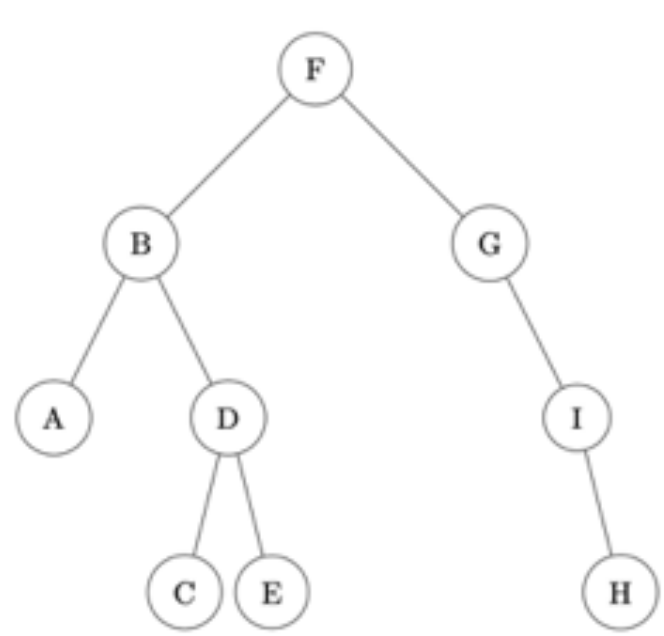
\includegraphics[width=8cm]{ressources/arbre.png}
    \end{center}
    \begin{enumerate}
        \item Construire le dictionnaire \textbf{\texttt{arbre}} représentant l'arbre binaire ci-dessus.
        \item Écrire la fonction récursive \textbf{\texttt{taille(arbre: dict, lettre: str) $\rightarrow$ int}} qui renvoie la taille de l'\texttt{\textbf{arbre}}. 
        \item Écrire à nouveau la fonction récursive \textbf{\texttt{taille(arbre: dict, lettre: str) $\rightarrow$ int}} en prenant en compte les 4 cas suivants: \begin{itemize}
            \item les deux fils du nœud sont '', 
            \item le fils gauche seulement est '', 
            \item le fils droit seulement est '', 
            \item aucun des deux fils n’est ''.
        \end{itemize}
    \end{enumerate}
\end{exo}
\begin{exo}
    \begin{enumerate}
        \item Écrire la fonction \texttt{\textbf{fusion}} prenant en paramètres deux tableaux non vides \texttt{\textbf{tab1}} et \texttt{\textbf{tab2}} d'entiers, chacun dans l’ordre croissant, renvoyant un tableau trié dans l’ordre croissant de l’ensemble des valeurs de \texttt{\textbf{tab1}} et \texttt{\textbf{tab2}}.
        \item Établir un jeu de tests permettant de vérifier la correction de la fonction.
    \end{enumerate}
\end{exo}
\begin{exo}
    On définit une classe gérant une adresse IPv4. On rappelle qu’une adresse IPv4 est une adresse de longueur 4 octets, notée en décimale à point, en séparant chacun des octets par un point. On considère un réseau privé avec une plage d’adresses IP de 192.168.0.0 à 192.168.0.255.
    On considère que les adresses IP saisies sont valides.
    Les adresses IP 192.168.0.0 et 192.168.0.255 sont des adresses réservées.
    \begin{enumerate}
        \item Compléter le code de la classe \texttt{\textbf{Adresse}} dans le fichier \texttt{\textbf{adresseip.py}}
        \item Créer plusieurs instances de la classe qui permettent de vérifier la correction des différentes méthodes.
    \end{enumerate}
\end{exo}
\begin{exo}
    Les chiffres romains sont un système ancien d’écriture des nombres. Les chiffres romains sont: I, V, X, L, C, D, et M.
    Ces symboles représentent respectivement 1, 5, 10, 50, 100, 500, et 1000 en base dix.\\
    Lorsque deux caractères successifs sont tels que:
    \begin{itemize}
        \item  le caractère placé à gauche possède une
        valeur supérieure ou égale à celui de droite, le nombre s’obtient en additionnant le caractère de
        gauche à la valeur de la chaîne située à droite.
        Ainsi, "XVI" est le nombre 16 car X + VI = 10 + 6.
        \item  le caractère placé à gauche possède une
        valeur strictement inférieure à celui de droite, le nombre s’obtient en retranchant le caractère de
        gauche à la valeur de la chaîne située à droite.
        Ainsi, "CDIII" est le nombre 403 car DIII – C = 503 – 100.
    \end{itemize}
    On dispose d’un dictionnaire \texttt{\textbf{dico}}, à compléter, où les clés sont les caractères apparaissant dans l’écriture en chiffres romains et où les valeurs sont les nombres entiers associés en
    écriture décimale.\\
    Compléter la fonction récursive \texttt{\textbf{rom\_to\_dec(nombre: str) $\rightarrow$ int}} du fichier \textbf{\texttt{romain.py}}, qui renvoie l'écriture décimale du paramètre \textbf{\texttt{nombre}} écrit en chiffres romains
\end{exo}
\end{document}